\documentclass[12pt,aspectratio=169]{beamer}

\usetheme{metropolis}
\setbeamertemplate{bibliography item}{\insertbiblabel}
\usepackage{xcolor}
\usepackage{appendixnumberbeamer}
\usepackage{verbatim}
\usepackage{caption}
\usepackage{minted}
\setsansfont[BoldFont={Fira Sans Bold}, ItalicFont={Fira Sans Italic}]{Fira Sans Regular}
\usepackage[backend=biber,style=ieee]{biblatex}
\usepackage{hyperref}
\usepackage{circuitikz}
\ctikzset{tripoles/pmos style/emptycircle}
\ctikzset{tripoles/mos style/arrows}
\graphicspath{{./figs/}}
\setlength{\belowcaptionskip}{-10pt}
\setbeamersize{text margin left=5mm,text margin right=7mm}

\title{EECS 151/251A: Discussion 2}
\subtitle{Noise Margins, RTL Design, Simulation}
\author{}
\date{9/5/2019}

\begin{document}
\begin{frame}
    \maketitle
\end{frame}

\begin{frame}{The CMOS Inverter}
  \begin{columns}
    \begin{column}{0.3\textwidth}
      \begin{center}
        \begin{circuitikz}[line width=1.25pt]
          %\draw[step=1cm,gray,very thin] (-1,-1) grid (6,6);
          \draw
            (0,0) node[nmos](n) {}
            (0,2) node[pmos](p) {}
            (p.S) to[short] ++(-0.5,0) to[short] ++(1,0)
            (p.S) node[anchor=south] {$V_{DD}$}
            (n.S) node[ground] {} ++(0,0)
            (p.D) -- (n.D)
            (p.G) -- (n.G)
            (-1,1) to[short,-o] ++(-0.5,0) node[anchor=east] {$V_{in}$}
            (n.D) ++(0,0.25) to[short,-o] ++(0.5,0) node[anchor=west] {$V_{out}$}
        ;\end{circuitikz}
      \end{center}
    \end{column}
    \begin{column}{0.6\textwidth}
      \begin{itemize}
        \setlength\itemsep{0.75em}
        \item NMOS turns `on' when $V_{in} > V_{th,n}$
        \item PMOS turns `on' when $V_{DD} - V_{in} > V_{th,p}$
        \item We assume each device has an on ($R_{on}$) and off ($R_{off}$) resistance
      \end{itemize}
    \end{column}
  \end{columns}
\end{frame}

\begin{frame}{Voltage Transfer Characteristic}
  \begin{columns}
    \begin{column}{0.5\textwidth}
      \begin{center}
        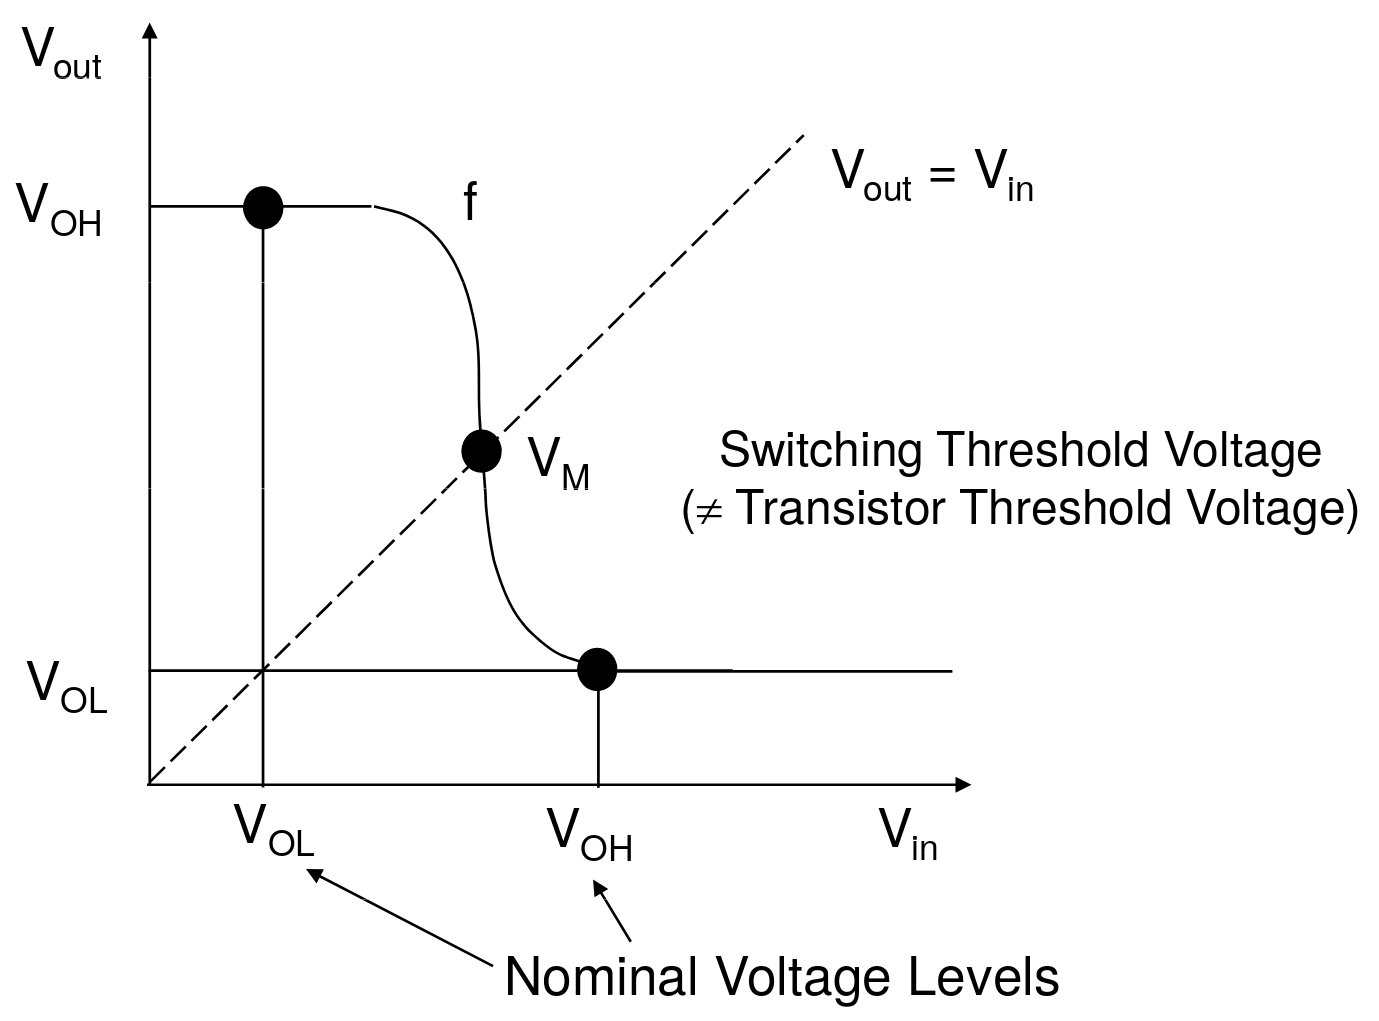
\includegraphics[width=\textwidth]{vtc.png}
      \end{center}
    \end{column}
    \begin{column}{0.5\textwidth}
      \begin{itemize}
        \setlength\itemsep{0.75em}
        \item $V_{OL} = 0$ and $V_{OH} = V_{DD}$ are the nominal low and high voltage levels
        \item $V_M$ - the switching threshold is a function of the relative `strength` of the NMOS and PMOS
        \item Draw a VTC for $V_{DD} = 1, V_{th,n} = 0.2, V_{th,p} = 0.3, R_{on,n}=10 k\Omega, R_{on,p}=20 k\Omega$
      \end{itemize}
    \end{column}
  \end{columns}
\end{frame}

\begin{frame}{Noise Margins}
  \begin{columns}
    \begin{column}{0.5\textwidth}
      \begin{center}
        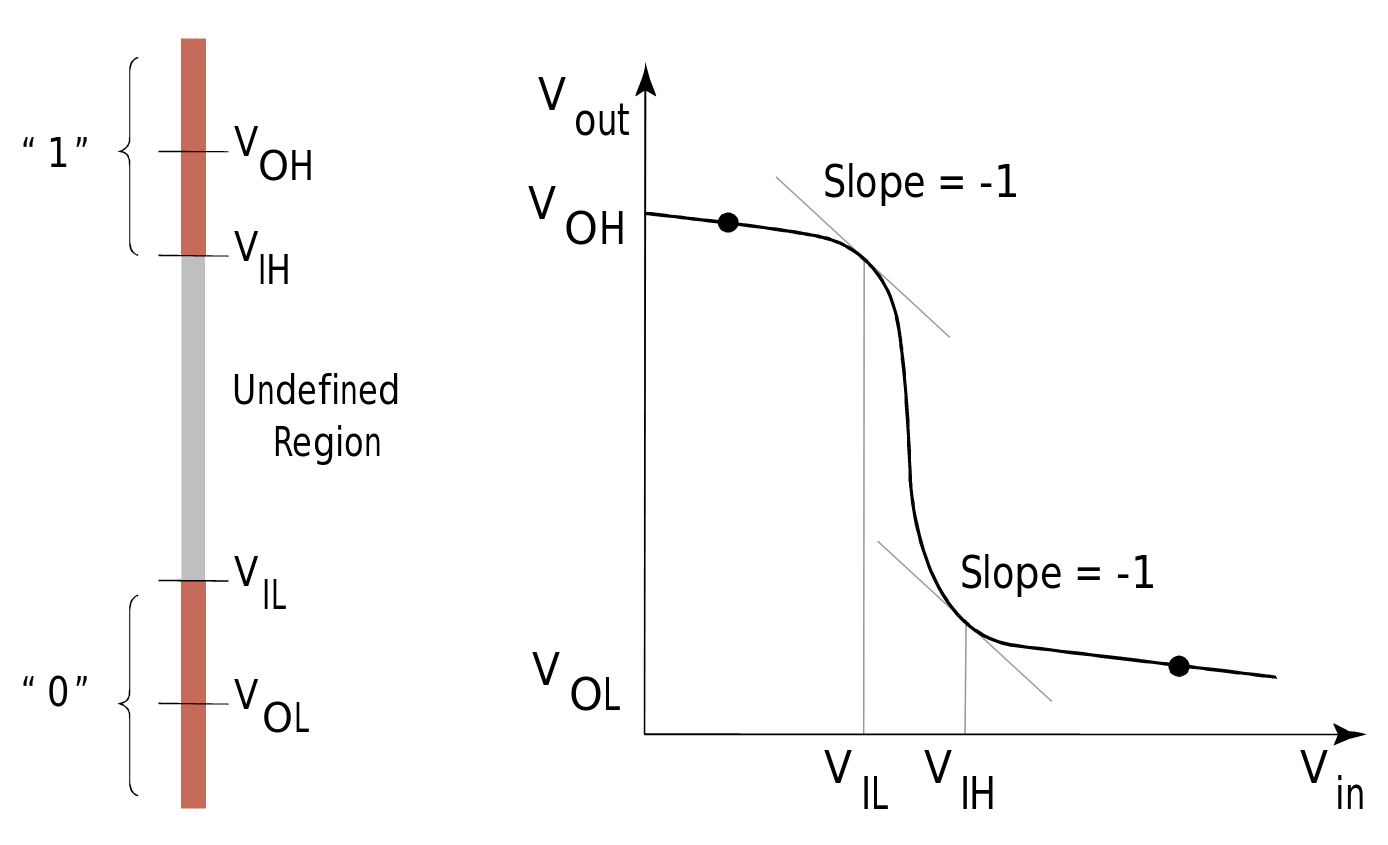
\includegraphics[width=\textwidth]{vtc_annotated.png}
      \end{center}
    \end{column}
    \begin{column}{0.5\textwidth}
      \begin{itemize}
        \setlength\itemsep{0.75em}
        \item $V_{IL}$ and $V_{IH}$ - bound the high-gain region of the VTC (unstable, high noise influence)
        \item In the undefined region the inverter acts like an amplifier and amplifies noise on the input and supply
      \end{itemize}
    \end{column}
  \end{columns}
\end{frame}

\begin{frame}{Regeneration}
  \begin{center}
    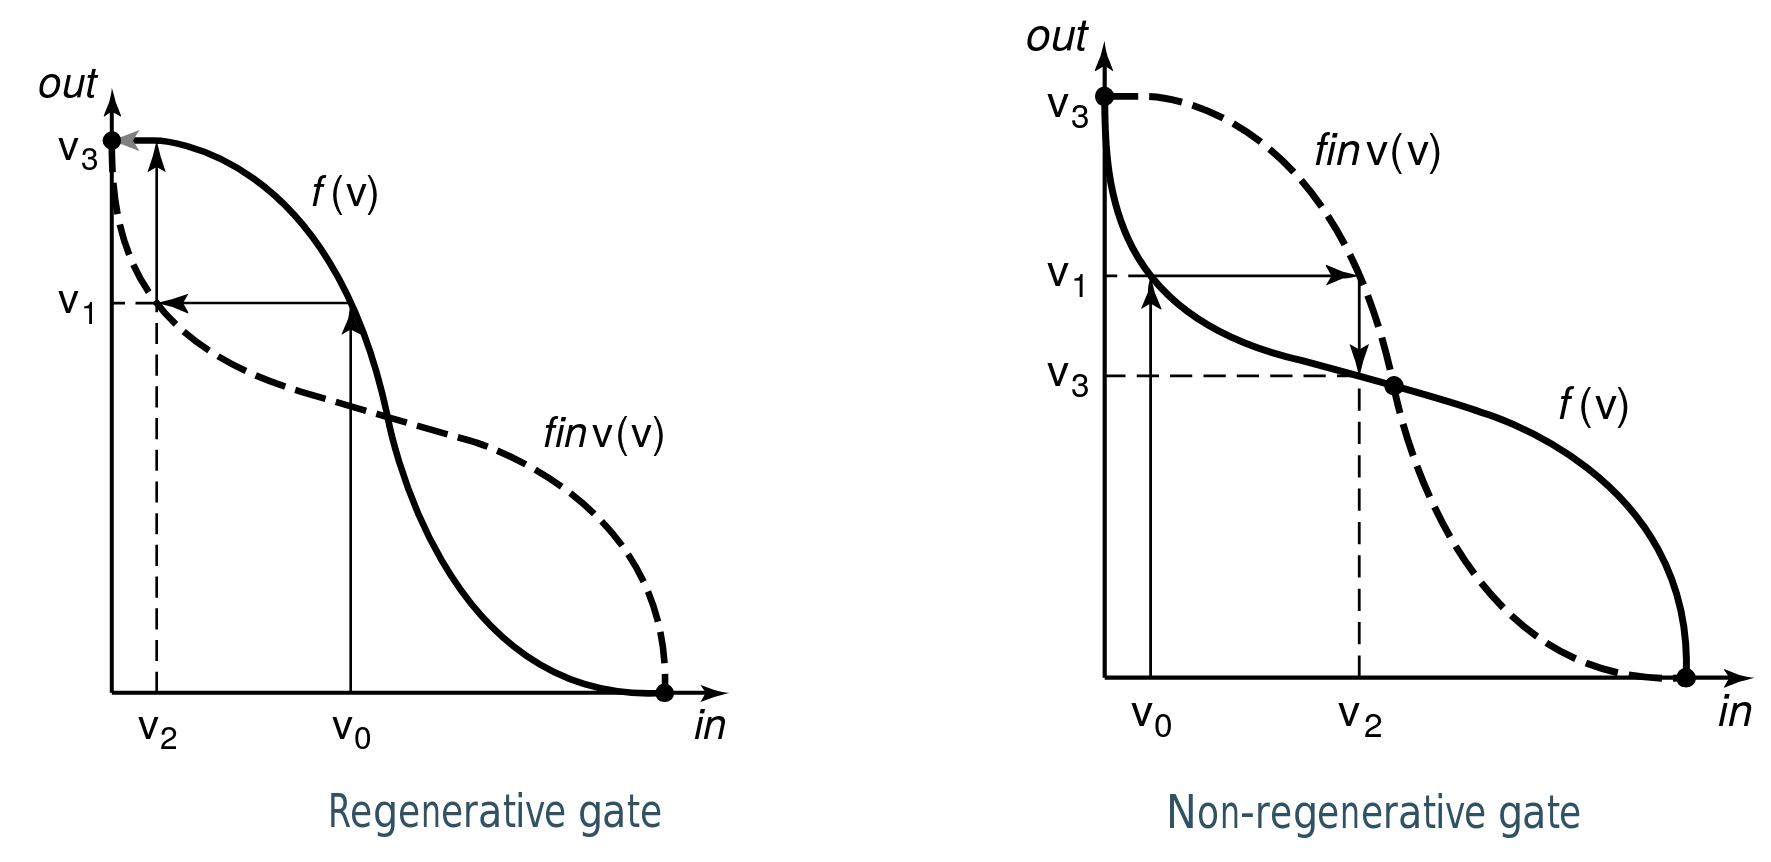
\includegraphics[width=0.7\textwidth]{regen.png}
  \end{center}
  \begin{itemize}
    \item Regenerative inverter has a VTC with low-gain regions around supplies and a high-gain region in between
  \end{itemize}
\end{frame}

\begin{frame}{Inverter Chain}
  \begin{columns}
    \begin{column}{0.5\textwidth}
      \begin{center}
        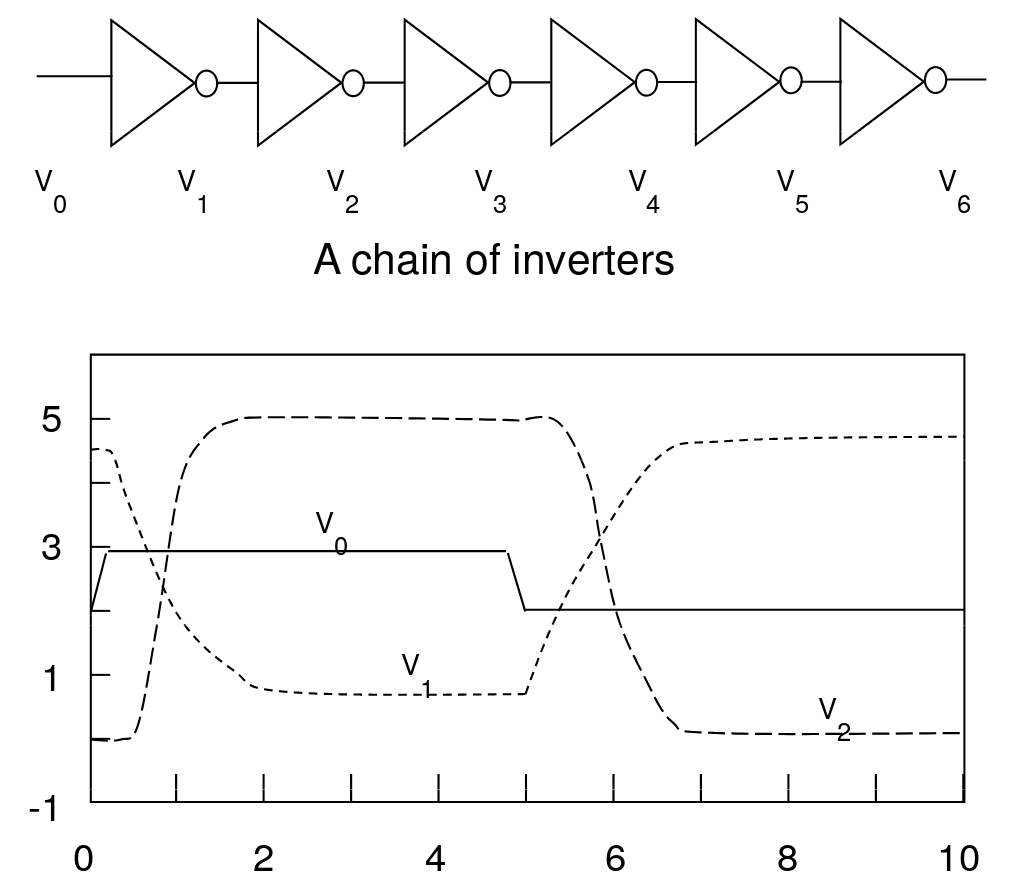
\includegraphics[width=\textwidth]{regen2.png}
      \end{center}
    \end{column}
    \begin{column}{0.5\textwidth}
      \begin{itemize}
        \setlength\itemsep{0.75em}
        \item A chain of CMOS inverters is regenerative, due to their VTCs
        \item As long as the input to the chain is not in the undefined region, the output will swing from rail to rail
      \end{itemize}
    \end{column}
  \end{columns}
\end{frame}

\begin{frame}{Verilog}
  \begin{itemize}
    \item We're going over the \href{http://inst.eecs.berkeley.edu/~eecs151/fa19/files/verilog/Verilog_Primer_Slides.pdf}{Verilog Primer Slides} and some slides from last semester's Verilog discussion.
  \end{itemize}
\end{frame}

\begin{frame}{Simulation}
  We can test RTL via simulation before putting it on the FPGA or fabricating an ASIC.

  Let's test a simple adder circuit (demo time), then a freerunning counter, and some other stuff.
\end{frame}

\end{document}
